\documentclass{article}
\usepackage[margin=1in]{geometry}
\usepackage{amsmath}
\usepackage{amssymb}
\usepackage{amsthm}
\usepackage{graphicx}
\usepackage{booktabs}
\usepackage{hyperref}
\usepackage{float}
\usepackage{caption}
\usepackage{subcaption}
\usepackage{tikz}
\usetikzlibrary{positioning}
%\usepackage{newtxtext,newtxmath} % Times-like font
\usepackage{mathpazo} % Palatino font
%\usepackage{libertinus} % Libertinus font
\usepackage{pgfplots}
\pgfplotsset{compat=1.17} % or 1.18, etc.
\usepackage{pgf-pie} % pie charts
\usepgfplotslibrary{statistics}
\usepackage{enumitem}
\usepackage{tcolorbox}
\tcbuselibrary{breakable}
\usepackage{fancyhdr}
\pagestyle{fancy}
\fancyhf{}

\theoremstyle{definition}
\newtheorem{definition}{Definition}[section]
\newtheorem{example}{Example}[section]
\newtheorem{properties}{Properties}[section]
\theoremstyle{plain}
\newtheorem{theorem}{Theorem}[section]

\newenvironment{flushlefttab}{
  \begin{flushleft}
  \begin{tabular}{@{} l p{0.75\textwidth} @{}}}
  {\end{tabular}
  \end{flushleft}}



\setlength{\parindent}{0pt}




\begin{document}
\begin{center}
    \LARGE {Statistical Inference Notes} \\
    \Large {Chapter 1: Probability Theory}
\end{center}
\bigskip

\tableofcontents


\newpage

\refstepcounter{section}
\section*{Probability Theory}
\addcontentsline{toc}{section}{Probability Theory}
``The subject of \textbf{probability theory} is the foundation upon which all of statistics is built, providing a means for modeling populations, experiments, or almost anything else that can be considered a random phenomenon. Through these models, statisticians are able to draw inferences about populations, inferences based on examination of only a part of the whole."
%\textbf{Probability theory} is the means for modeling populations, experiments, or anything else that can be considered a random phenomenon, through which we can draw inferences based on examination of only part of the whole.
\bigskip


\subsection*{Set Theory}
\addcontentsline{toc}{subsection}{Set Theory}
\begin{definition}
    The set $S$ of all possible outcomes of a particular experiment is called the \textbf{sample space} of the experiment.
\end{definition}

\begin{example}
    ${H, T}$ is the sample space for flipping a coin.
    ${2, 3, ..., 11, 12}$ is the sample space for the rolling of two dice.
\end{example}

A sample space may be countable or uncountable. The above are two examples of countable sample spaces, while examples of an \textit{un}countable sample space might include $S = [0, 1]$ for the generation of a random number between 0 and 1, or $[0, \inf)$ representing the distance traveled by some particle in an experiment.
\nextp

\begin{definition}
    An \textbf{event} $A$ is any collection of possible outcomes of an experiment, i.e., any subset of $S$. $A$ is said to occur if the outcome of the experiment is in the set $A$.
\end{definition}

\begin{properties}
    Let $A$ and $B$ be any two sets (events). The following are some useful characteristics of sets.
    \begin{itemize}
        \item \textbf{Containment}: $A \subset B \iff x \in A \implies x \in B$
        \item \textbf{Equality}: $A = B \iff A \subset B \mathrm{\ and\ } B \subset A$
        \item \textbf{Union}: $A \cup B = \{x: x \in A \mathrm{\ or\ } x \in B\}$
        \item \textbf{Intersection}: $A \cap B = \{x: x \in A \mathrm{\ and\ } x \in B\}$
        \item \textbf{Complement}: $A^c = \{x: x \notin A\}$
    \end{itemize}
\end{properties}

\begin{theorem}
    For any events $A, B, C$ defined on a sample space $S$, the following properties hold: \\
    \begin{center}
    \begin{tabular}{@{} l l}
        \textbf{Commutativity:} &
        $\begin{aligned}
            A \cup B &= B \cup A \\
            A \cap B &= B \cap A
        \end{aligned}$ \\[3ex]
    
        \textbf{Associativity:} &
        $\begin{aligned}
            A \cup (B \cup C) &= (A \cup B) \cup C \\
            A \cap (B \cap C) &= (A \cap B) \cap C
        \end{aligned}$ \\[3ex]
    
        \textbf{Distributive Laws:} &
        $\begin{aligned}
            A \cap (B \cup C) &= (A \cap B) \cup (A \cap C) \\
            A \cup (B \cap C) &= (A \cup B) \cap (A \cup C)
        \end{aligned}$ \\[3ex]
    
        \textbf{De Morgan's Laws:} &
        $\begin{aligned}
            (A \cup B)^c &= A^c \cap B^c \\
            (A \cap B)^c &= A^c \cup B^c
        \end{aligned}$
    \end{tabular}
    \end{center}
\end{theorem}

We can also extend the notions of union and intersection to infinite collections of sets $A_1, A_2, \dots$:
\begin{align*}
    & \bigcup_{i=1}^{\infty}A_i = \{x \in S: x \in A_i \mathrm{\ for\ some\ } i\} \\
    & \bigcap_{i=1}^{\infty}A_i = \{x \in S: x \in A_i \mathrm{\ for\ all\ } i\} 
\end{align*}
\nextp

\textit{Note:} We denote with $\emptyset$ the \textbf{empty set}, i.e., the set having no elements in it.

\begin{definition}
    Two events $A$ and $B$ are \textbf{disjoint}, or \textbf{mutually exclusive}, if $A \cap B = \emptyset$. The events $A_1, A_2, \dots$ are \textbf{pairwise disjoint} if $A_i \cap A_j = \emptyset$ for all $i \neq j$.
\end{definition}

\begin{definition}
    If $A_1, A_2, \dots$ are pairwise disjoint and $\cup_{i=1}^{\infty}A_i = S$, then we say that $A_1, A_2, \dots$ form a \textbf{partition} of $S$.
\end{definition}

\begin{example}
    The most obvious partition of $S$ would be the sets $\{A, A^c\}$ for any event $A$. (This may seem rather pointless but we will revisit its use later when discussing Bayes' Theorem.)
\end{example}
\bigskip

\subsection*{Basics of Probability Theory}
\addcontentsline{toc}{subsection}{Basics of Probability Theory}
To begin this section we outline the \textit{very basic} facets of measure theory, which provide the under-the-hood mechanisms with which we can formally define and talk about probability.
\begin{definition}
    A collection of subsets of $S$ is a \textbf{sigma algebra}, or \textbf{Borel field}, denoted by $\mathcal{B}$, if it satisfies the following properties:
    \begin{itemize}
        \item $\emptyset \in \mathcal{B}$
        \item If $A \in \mathcal{B}$, then $A^c \in \mathcal{B}$ \quad (closed under complementation)
        \item If $A_1, A_2, \dots \in \mathcal{B}$, then $\cup A_i \in \mathcal{B}$ \quad (closed under countable unions)
    \end{itemize}
\end{definition}

\begin{example}
    The simplest example of a sigma algebra is the \textbf{trivial sigma algebra}, $\{\emptyset, S\}$.
\end{example}

\begin{example}
    If $S$ is finite or countable, we can take $\mathcal{B} = \{\mathrm{all\ subsets\ of\ } S\}$.
\end{example}

\begin{example}
    If $S$ is uncountable, we may take $\mathcal{B} = $ all sets of the form $[a,b], [a,b),(a,b], (a,b)$
\end{example}
\nextp

Usually we'll just take $\mathcal{B}$ to be the simplest sigma algebra possible: the smallest one containing all open sets in a given sample space $S$. 
Now we may take a look at defining probability...
\begin{definition}
    Let $S$ be a sample space with an associated sigma algebra $\mathcal{B}$. A \textbf{probability function} is a function $P$ with domain $\mathcal{B}$ satisfying
    \begin{itemize}
        \item $P(A) \geq 0$ for all $A \in \mathcal{B}$
        \item P(S) = 1
        \item If $A_1, A_2, \dots \in \mathcal{B}$ are pairwise disjoint, then $P(\bigcup_{i=1}^{\infty}{A_i}) = \sum_{i=1}^{\infty}{P(A_i)}$
    \end{itemize}
    These conditions are known as the Axioms of Probability, or the Kolmogorov Axioms. In particular, the last axiom is known as the Axiom of Countable Additivity.
\end{definition}
\nextp

In practice, we don't want to always check these axioms to verify whether a function is a valid probability function. The below result helps in this regard by giving a systematic way to confirm a valid probability function.
\begin{theorem}
    Let $S = \{s_1, \dots, s_n\}$ be a finite set and let $\mathcal{B}$ be any sigma algebra of sets of $S$. Also let $p_1, \dots, p_n$ be nonnegative integers that sun to $1$. For any $A \in \mathcal{B}$, let $P(A)$ be defined by
    \[
    P(A) = \sum_{i: s_i \in A}{p_i}
    \]
    Then, $P$ is a probability function on $\mathcal{B}$.
\end{theorem}
\nextp

There are many important properties of probability functions as well as relations we can make between multiple events that will allow us to find probability values for events. We outline these now.

\begin{theorem}
    Let $P$ be a probability function and let $A \in \mathcal{B}$ be an event. Then:
    \begin{itemize}
        \item $P(\emptyset) = 0$
        \item $P(A) \leq 1$
        \item $P(A^c) = 1 - P(A)$
    \end{itemize}
\end{theorem}

\begin{theorem}
    Let $P$ be a probability function and let $A, B \in \mathcal{B}$ be any events. Then:
    \begin{itemize}
        \item $P(A \cap B^c) = P(A) - P(A \cap B)$
        \item $P(A \cup B) = P(A) + P(B) - P(A \cap B)$
        \item $If A\subset B$, then $P(A) \leq P(B)$
    \end{itemize}
\end{theorem}

\begin{corollary}
    For any events $A, B \in \mathcal{B}$, 
    \[
    P(A \cap B) \geq P(A) + P(B) - 1
    \]
    This result is known as Bonferroni's inequality and is useful for bounding the probability of the intersection of two events, using the probabilities of the individual events.
\end{corollary}

\begin{theorem}
    Let $P$ be a probability function. Then:
    \begin{itemize}
        \item $P(A) = \sum_{i=1}^{\infty}{A \cap C_i}$ for any partition $C_1, C_2, \dots$
        \item $P\left(\bigcup_{i=1}^{\infty}{A_i}\right) \leq \sum_{i=1}^{\infty}{P(A_i)}$ for any sets $A_1, A_2, \dots$ \quad (Boole's inequality)
    \end{itemize}
\end{theorem}
\nextp

We can apply Boole's inequality above to the event $A^c$ and obtain an expanded version of Bonferroni's inequality, in more general terms, in the following way:
\[
P\left(\bigcup_{i=1}^{\infty}{A_i^c}\right) \leq \sum_{i=1}^{\infty}{P(A_i^c)}
\]
Now, note that $P(A_i^c) = 1 - P(A_i)$ and $\cup{A_i^c} = (\cap{A_i})^c$. Then, 
\begin{align}
    & 1 - P\left(\bigcap_{i=1}^{\infty}{A_i}\right) \leq n -\sum_{i=1}^{\infty}{P(A_i)} \\
    & P\left(\bigcap_{i=1}^{\infty}{A_i}\right) \geq \sum_{i=1}^{\infty}{P(A_i)} - (n - 1)
\end{align}
\nextp

Now we move on to the topic of counting, which is used for constructing probability assignments on finite sample spaces as well as other tasks.

\begin{theorem}[\textbf{Fundamental Theorem of Counting}]
    Suppose that a ``job" consists of $k$ separate tasks where the $i$th task can be done in $n_i$ different ways, for $i = 1, \dots, k$. Then, the entire job can be done in $n_1 \times \dots \times n_k$ ways.
\end{theorem}

While this theorem can be used for basic examples, usually we must make a couple distinctions depending on the problem at hand. Namely, we must differentiate between counting with versus without replacement, and between the cases where ordering does and does not matter to the outcome. We can arrange the following table of the number of possible arrangements of size $r$ from $n$ objects.
\begin{center}
\begin{tabular}{c|c|c}
 & without replacement & with replacement \\
\hline
Ordered & $\frac{n!}{r!(n-r)!}$ & $n^r$ \\
\hline
Unordered & $\binom{n}{r}$ & $\binom{n+r-1}{r}$ \\
\end{tabular}
\end{center}
\nextp

If we have equally likely outcomes in $S$, then we can use the above to count the number of outcomes in a given event $A$ to find $P(A)$:
\[
P(A) = \sum_{s_i \in A}{P(\{s_i\})} = \sum_{s_i \in A}{\frac{1}{N}} = \frac{\text{number of elements in } A}{\text{number of elements in } S}
\]

\begin{example}
    Find the probability of various poker hands.
    \[
    P(\text{4 of a kind}) = \frac{13 \times 48}{\binom{52}{5}} = 
    \]
\end{example}
\bigskip


\subsection*{Conditional Probability and Independence}
\addcontentsline{toc}{subsection}{Conditional Probability and Independence}
The notion of conditional probability will allow us to update our sample space at hand based on new information/data. For example, to find the probability of drawing 4 aces from a deck of cards, we can say $P(4 \text{ aces}) = \frac{4}{52} \times \frac{3}{51} \times \frac{2}{50} \times \frac{1}{49}$, where with each term we are updating the sample space of possible cards we may draw from, using the knowledge of the card(s) just drawn.

\begin{definition}
    If $A$ and $B$ are events in $S$, where $P(B) > 0$, then the conditional probability of $A$ given $B$ is given by:
    \[
    P(A \vert B) = \frac{P(A \cap B)}{P(B)}
    \]
\end{definition}

Applying the above definition, we can also conveniently write probabilities of intersections, with
\[
P(A \cap B) = P(A \vert B)P(B) = P(B \vert A)P(A)
\]

\begin{theorem}[\textbf{Bayes' Theorem}]
    Let $A, B$ be sets in $S$. Then,
    \[
    P(A \vert B) = \frac{P(A)P(B \vert A)}{P(B)}
    \]
    In general, let $A_1, A_2, \dots$ be a partition of $S$ and $B$ be any event set. Then,
    \[
    P(A_i \vert B) = \frac{P(A_i)P(B \vert A_i)}{\sum_{j=1}^{\infty}{P(A_j)P(B \vert A_j)}}
    \]
\end{theorem}

\begin{definition}
    Events $A$ and $B$ are statistically independent if
    \[
    P(A \cap B) = P(A)P(B) \iff P(A \vert B) = P(A) \iff P(B \vert A) = P(B) 
    \]
\end{definition}

\begin{theorem}
    Let $A$ and $B$ be independent events. Then, the following pairs of events are also independent:
    \begin{itemize}
        \item $A$ and $B^c$
        \item $A^c$ and $B$
        \item $A^c$ and $B^c$
    \end{itemize}
\end{theorem}

\begin{definition}
    A collection of events $A_1, \dots, A_n$ are mutually independent if for any subcollection of events $A_{i_1}, \dots, A_{i_k}$, we have:
    \[
    P\left(\bigcap_{j=1}^{k}{A_{i_j}}\right) = \prod_{j=1}^{k}{P(A_{i_j})}
    \]
\end{definition}
\bigskip


\subsection*{Random Variables}
\addcontentsline{toc}{subsection}{Random Variables}
\begin{definition}
    A random variable $X$ is a function from a sample space $S$ into $\mathbb{R}$
\end{definition}

Suppose that we have a sample space $S = \{s_1, \dots, s_n\}$ with a probability function $P$ and we define a new random variable $X$ with range $\mathcal{X} = \{x_1, \dots, x_m\}$. Then, we can define a probability function $P_X$ on $\mathcal{X}$ with:
\[
P_X(X = x_i) =P(\{s_j \in S: X(s_j) = x_i\})
\]
We say that $P_X$ is an \textit{induced} probability function on $\mathcal{X}$.

\begin{example}
    Consider an experiment involving flipping a coin three times and define the random variable $X$ to be the number of heads in those 3 rolls. Then, we have the following:
    \begin{center}
    \begin{tabular}{c | c c c c c c c c}
    $s$ & HHH & HHT & HTH & THH & TTH & THT & HTT & TTT \\
    \midrule
    $X(s)$ & 3 & 2 & 2 & 2 & 1 & 1 & 1 & 0 \\
    \end{tabular}
    \end{center}
    The induced probability function $P_X$ will be given by:
    \begin{center}
    \begin{tabular}{c | c c c c}
    $x$ & 0 & 1 & 2 & 3 \\
    \midrule
    $P_X(X = x)$ & $\dfrac{1}{8}$ & $\dfrac{3}{8}$ & $\dfrac{3}{8}$ & $\dfrac{1}{8}$ \\
    \end{tabular}
    \end{center}
    \label{ex:probab_func}
\end{example}

The above were for the case where $S$ and $\mathcal{X}$ are finite or countable. We can define $P_X$ for an uncountable $\mathcal{X}$ similarly. For any set $A\subset \mathcal{X}$,
\[
P_X(X \in A) = P(\{s\in S: X(s) \in A\})
\]


\subsection*{Distribution Functions}
\addcontentsline{toc}{subsection}{Distribution Functions}
\begin{definition}
    The cumulative distribution function (cdf) of a random variable $X$ is defined by:
    \[
    F_X(x) = P_X(X \leq x)
    \]
    for all $x$.
\end{definition}
\nextp

\begin{figure}[h!]
\centering
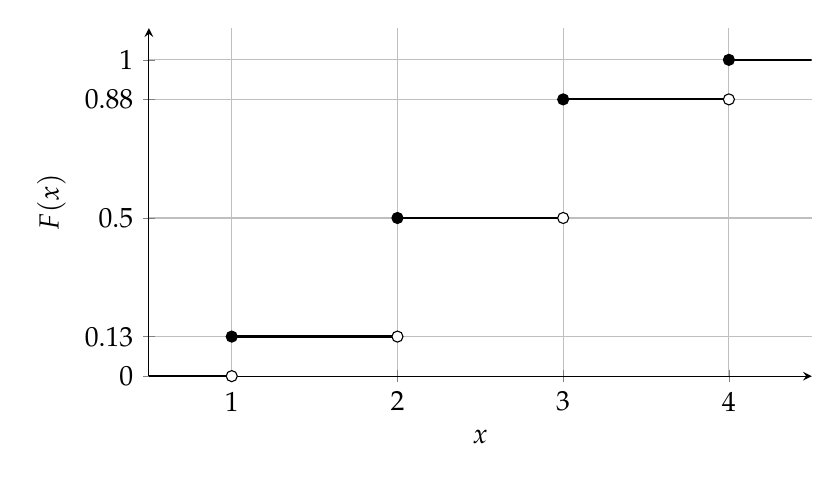
\begin{tikzpicture}
\begin{axis}[
    axis lines=left,
    xlabel={$x$},
    ylabel={$F(x)$},
    ymin=0, ymax=1.1,
    xmin=0.5, xmax=4.5,
    xtick={1,2,3,4},
    ytick={0,0.125,0.5,0.875,1},
    grid=both,
    width=10cm,
    height=6cm
]

% Horizontal lines (no vertical lines)
\addplot[black, thick] coordinates {(0.5, 0) (1, 0)};
\addplot[black, thick] coordinates {(1, 0.125) (2, 0.125)};
\addplot[black, thick] coordinates {(2, 0.5) (3, 0.5)};
\addplot[black, thick] coordinates {(3, 0.875) (4, 0.875)};
\addplot[black, thick] coordinates {(4, 1) (4.5, 1)};

% Solid dots for included (right-continuous) values
\addplot[only marks, mark=*, mark options={fill=black}, black]
coordinates {(1, 0.125) (2, 0.5) (3, 0.875) (4, 1)};

% Open dots for left limits
\addplot[only marks, mark=*, mark options={fill=white}, black]
coordinates {(1, 0) (2, 0.125) (3, 0.5) (4, 0.875)};

\end{axis}
\end{tikzpicture}
\caption{Cumulative distribution function (cdf) of Example \ref{ex:probab_func}}
\label{fig:cdf-discrete}
\end{figure}

%Note: The cdf is \textit{right-continuous}.
\nextp

\begin{theorem}
    The function $F_X(x)$ is a cdf if and only if the following hole:
    \begin{itemize}
        \item $\lim_{x \rightarrow -\infty}{F(x)} = 0$ and $\lim_{x \rightarrow \infty}{F(x)} = 1$
        \item F(x) is a nondecreasing function
        \item F(x) is right-continuous, i.e., $\lim_{x \rightarrow x_0^+}{F(x)} = F(x_0)$ for any $x_0$
    \end{itemize}
\end{theorem}
\nextp

\begin{example}
    Consider an experiment where we flip a coin until we get a heads. (TO DO: Example 1.5.4)
\end{example}
\nextp

\begin{definition}
    A random variable $X$ is continuous if $F_X(x)$ is a continuous function and discrete if $F_X(x)$ is a step function.
\end{definition}

\begin{definition}
    Let $\mathcal{B}$ be the smallest sigma algebra containing all the intervals of real numbers of the form $[a,b], [a,b),(a,b], (a,b)$. The random variables $X$ and $Y$ are identically distributed if for all $A \in \mathcal{B}$, $P(X\in A) = P(Y\in A)$
\end{definition}

\begin{example}
    If we revisit the experiment of flipping a coin 3 times and define the random variables $X =$ number of heads and $Y =$ number of tails, then $X$ and $Y$ are identically distributed (even though we don't have $X(s) = Y(s)$ for any sample $s \in S$).
\end{example}

\begin{theorem}
    The random variables $X$ and $Y$ are identically distributed if and only if $F_X(x) = F_Y(x)$ for all $x$.
\end{theorem}
\bigskip


\subsection*{Density and Mass Functions}
\addcontentsline{toc}{subsection}{Density and Mass Functions}
\begin{definition}
    The probability mass function (pmf) of a discrete random variable $X$ is given by
    \[
    f_X(x) = P(X= x) \quad \text{ for all } x
    \]
\end{definition}

\begin{definition}
    The probability density function (pdf) of a continuous random variable $X$ is the function $f_X(x)$ that satisfies 
    \[
    F_X(x) = \int_{-\infty}^{x}{f_X(t)dt} \quad \forall x
    \]
    Naturally, we also have the relationship $\frac{d}{dx}F_X(x)= f_X(x)$
\end{definition}

Notation: If $X$ follows a distribution given by the cdf $F_X$, we write $X \sim F_X(x)$. Likewise, we may also write $X \sim f_X(x)$. Lastly, if $X$ follows the same distribution as another random variable $Y$, then we could write $X\sim Y$.
\nextp

We can use the relationship between the cdf and pdf to find probabilities.
\[
P(a \leq X \leq b) = F_X(b) - F_X(a) = \int_{a}^{b}{f_X(x)dx}
\]

For a continuous random variable $X$, we will have $P(X = x) = 0$ for all $x$. So, for some points $a, b \in S$, we have that
\[
P(a < X < b) = P(a < X \leq b) = P(a \leq X < b) = P(a \leq X \leq b)
\]

\clearpage
\begin{figure}[htbp]
\centering
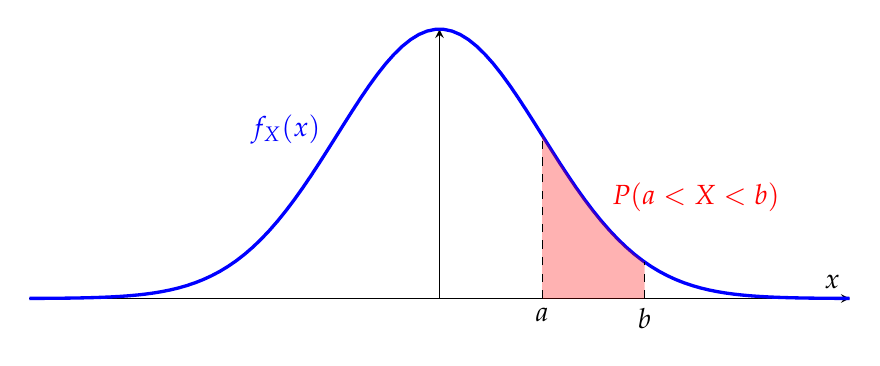
\begin{tikzpicture}
  \begin{axis}[
    domain=-5:5,
    samples=100,
    axis lines=middle,
    xlabel={$x$},
    ylabel=\empty,
    xtick=\empty,
    ytick=\empty,
    enlargelimits=false,
    clip=false,
    grid=major,
    width=12cm,
    height=5cm,
  ]

  % Normal density curve
  \addplot [very thick, blue, domain=-4:4] {1/sqrt(2*pi) * exp(-x^2/2)};
  
  % Shaded area from a to b
  \addplot [
    draw=none,
    domain=1:2,
    fill=red,
    fill opacity=0.3
  ] {1/sqrt(2*pi) * exp(-x^2/2)} \closedcycle;

  % Vertical lines for a and b
  \addplot[dashed] coordinates {(1,0) (1,{1/sqrt(2*pi) * exp(-1^2/2)})};
  \addplot[dashed] coordinates {(2,0) (2,{1/sqrt(2*pi) * exp(-2^2/2)})};

  \node[below] at (axis cs:1,0) {$a$};
  \node[below] at (axis cs:2,0) {$b$};
  \node[blue] at (axis cs:-1.5,0.25) {$f_X(x)$};
  \node[red] at (axis cs:2.5,0.15) {$P(a < X < b)$};
  
  \end{axis}
\end{tikzpicture}
\caption{Probability using area under the density curve $f_X(x)$.}
\label{fig:area-under-normal-pdf}
\end{figure}
\bigskip

\begin{theorem}
    A function $f_X(x)$ is a pdf/pmf of a random variable $X$ if and only if:
    \begin{itemize}
        \item $f_X(x) \geq 0 \quad \forall x$
        \item $\sum_{x}{f_X(x)} = 1$ if $f_X$ is a pmf; $\int_{-\infty}^{\infty}{f_X(x)dx} = 1$ if $f_X$ is a pdf.
    \end{itemize}
\end{theorem}




\end{document}